\documentclass[b5paper,fleqn]{ltjsarticle}
\usepackage{tkz-berge}
\newcommand\s[1]{\subsection*{#1}\noindent\ignorespaces}
\newcommand\sbs[1]{\subsubsection*{#1}}
\newcommand\al[1]{\begin{align*}#1\end{align*}}
\newcommand\tx{\intertext}
\renewcommand{\labelenumi}{\alph{enumi}).}
\title{オートマトンと言語}
\author{大阪分散技術コミュニティ}
\begin{document}
\maketitle

\begin{description}
\item [タイトル] オートマトンと言語
\item [著者] Michael Sipser
\item [訳者] 太田和夫,田中圭介
\item [出版日] 2008/5/21
\item [出版社] 共立出版
\item [ISBN10] 4320122070
\item [ISBN13] 978-4320122079
\item [ページ数] 240
\item [言語] ja
\item [内容]MIT屈指の名講義の講義ノートをまとめた書
\end{description}

\section{Turing machine}
Turing機械に対して、Mの言語(the language of M)を
\[L(M)=\{\omega\in\Sigma^*|M(\omega)=accept\}\]
によって定義する。
\subsection{Turing-recognizable}
言語$L$が認識可能とは、あるTuring機械Mが存在し、$L(M)=L$となることである。
\subsection{Turing-decidable}
Turing機械$M$が判定装置(decider)であるとは
\[\forall\omega\in\Sigma^*, M(\omega)\neq loop\]
となることである。\par
言語$L$が判定可能とは、$L$が認識可能かつ$M$が判定装置であることである。

\section{Annotation}

\s{p15,---をつなげてるとき、その有向グラフを
強連結(strongly connected)という.}
正確な定義は任意の2点間に有向路(directed path)が存在することである。
例えば図0.16だと頂点は繋がっているが(connected)、3から6は
辿ることができない。よって強連結(strongly connected)とは言えない。

\section{Questions}
\s{p30,演習}\vskip-5pt
\sbs{0.1}
\begin{enumerate}
\renewcommand{\labelenumi}{\alph{enumi}).}
\item 奇数
\item 負を含む偶数
\item 偶数
\item 偶数かつ奇数
\item $\{(0,0),(0,1),(1,0),(1,1)\}$
\item $\emptyset$
\end{enumerate}
\sbs{0.2}
\begin{enumerate}
\item $\{1,10,100\}$
\item $\{m\in\mathcal{Z}|m>5\}$
\item $\{n\in\mathcal{N}|n<5\}$
\item $\{abc\}$
\item $\{\epsilon\}$
\item $\emptyset$
\end{enumerate}
\sbs{0.3}
\begin{enumerate}
\item はい。
\item いいえ。
\item $\{x,y,z\}$
\item $\{x,y\}$
\item $\{(x,x),(x,y),(y,x),(y,y),(z,x),(z,y)\}$
\item $\{\{x,y\},\{x\},\{y\},\emptyset\}$
\end{enumerate}
f). 集合Bの冪集合(power set)は$2^B$という記号で表すことが多い。
\sbs{0.4}
$a\times b$
\sbs{0.5}
$2^c$
\sbs{0.6}
\begin{enumerate}
\item 7
\item $X,Y$
\item 6
\item $X\times X, Y$
\item 8
\end{enumerate}
\sbs{0.7}
\begin{enumerate}
\item 例えば、$a=a'$ or $b=b'$によって関係$R$を定めると
\item b
\item b
  math\'ematicha
\end{enumerate}
\sbs{0.8}
pandax宿題
\sbs{0.9}

pandax宿題
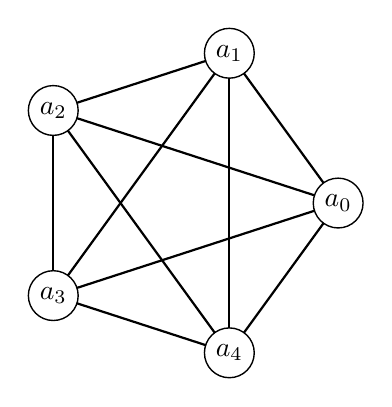
\begin{tikzpicture}
\SetVertexMath
\grComplete[RA=2]{5}
\end{tikzpicture}

\end{document}
